\chapter{Details of A Solution}
\section{About CERT C Secure Coding Standard }
The CERT C Secure Coding Standard provides rules and recommendations (collectively called guidelines) for secure coding in the C programming language. The goal of these rules and recommendations is to develop safe, reliable, and secure systems. Conformance to the coding rules defined in this standard are necessary (but not sufficient) to ensure the safety, reliability, and security of software systems developed in the C programming language. It is also necessary, for example, to have a safe and secure design. Safety-critical systems typically have stricter requirements than are imposed by this coding standard, for example requiring that all memory be statically allocated. However, the application of this coding standard will result in high-quality systems that are reliable, robust, and resistant to attack.

\subsection{Issues Not Addressed}
The following issues are not addressed by this standard:
\begin{itemize}
	\item \textbf{Design and Architecture.} Design level vulnerabilities are one of the dangerous ones. There are many standards to avoid design level vulnerabilities. This standard assumes that the product is free of design-level vulnerabilities
	
	\item \textbf{Coding Style.} Coding style issues are subjective; it has proven impossible to develop a
	consensus on appropriate style rules. This standard doesn't provide any coding styles.The easiest way to consistently apply a coding style is with the
	use of a code formatting tool. 
	
	\item \textbf{Tools.} SEI-CERT team didn't recommend  a particular vendors or
	tools.The developer can choose tools to enforce these rules.
	\item \textbf{ Controversial Rules} In general, the CERT secure coding standards try to avoid the
	inclusion of controversial rules that lack a broad consensus.
\end{itemize}
\subsection{Identifiers}
Each rule has a unique identifier, consisting of three parts:
\begin{itemize}
	\item \textbf{A three-letter mnemonic}, representing the section of the standard, is used to group similar rules and make them easier to find.
	\textit{eg: PRE: for preprocessor}
	\item \textbf{A two-digit numeric value} in the range of 00 to 99, which ensures each rule has a unique identifier.
	\textit{eg: PRE30}
	\item \textbf{The letter J/C}, which indicates that this is a Java language/C language rule and is included to prevent ambiguity with similar rules in CERT secure coding standards for other languages.
	\textit{eg: PRE30-C}
	Finally, the rule looks like,
	\textit{eg: PRE30-C - Do not create a universal character name through concatenation}
\end{itemize}

\subsection{Priority and Levels}
Each rule has an assigned priority. Priorities are assigned using a metric based on Failure
Mode, Effects, and Criticality Analysis. Three values are assigned
for each rule on a scale of 1 to 3 for
\newline
\newline
\textbf{ Severity} How serious are the consequences of the rule being ignored:
\begin{itemize}
\item 1 = low  
The effect is denial-of-service attack, abnormal termination 
\item 2 = medium 
The effect is data integrity violation, unintentional information disclosure)
\item 3 = high 
The effect is run arbitrary code, privilege escalation)
\end{itemize}

\textbf{Likelihood} The probability that a flaw introduced by violating the rule could lead to an exploitable vulnerability:
\begin{itemize}
\item 1 = unlikely
\item 2 = probable
\item 3 = likely
\end{itemize}

\textbf{Remediation cost} How expensive is it to remediate existing code to comply with the rule:
\begin{itemize}
\item 1 = high
The effect is manual detection and correction.
\item 2 = medium
The effect is automatic detection and manual correction.
\item 3 = low
The effect is automatic detection and correction.
\end{itemize}
The three values are multiplied together for each rule. This product provides a measure to prioritize the rules. These products range from 1 to 27. Rules with a priority in the range of 1 to 4 are level 3 rules, 6 to 9 are level 2, and 12 to 27
are level 1. As a result, it is possible to claim level 1, level 2, or complete compliance (level 3)
with a standard by implementing all rules in a level, as shown in Figure \ref{fig:1}\cite{cert-c}
	\begin{figure}[H]
		
		
		\centering
		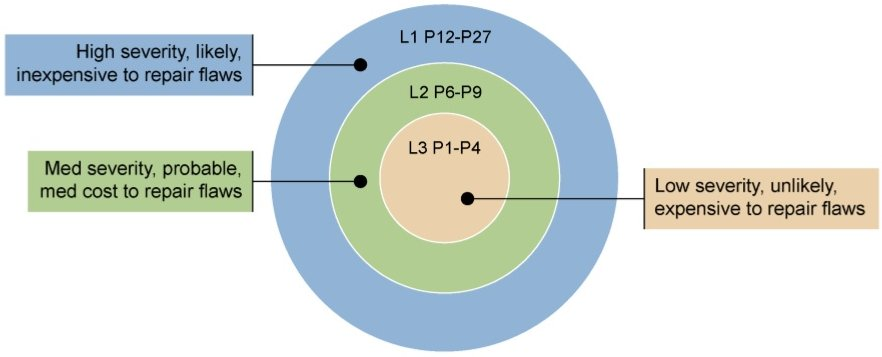
\includegraphics[width=.9\linewidth]{Figures/lev}
		\caption{Levels and priority ranges}	 
		\label{fig:1}
		
	\end{figure}
	 
\subsection{Rules and Recommendations}
Rules are normalized ones. It is mandatory to follow rules.Rules must meet the following criteria:
	\begin{enumerate}
	 
		\item Violation of the guideline is likely to result in a defect that may adversely affect the safety, reliability, or security of a system
		\item The guideline does not rely on source code annotations or assumptions.
	Rules are identified by the label rule.
\end{enumerate}
		Recommendations are not normalized. Recommendations are suggestions for improving code quality.It is not mandatory to follow recommendations Guidelines are defined to be recommendations when all of the following conditions are met:
	\begin{enumerate}
	  
		\item Application of a guideline is likely to improve the safety, reliability, or security of software systems.
	\item One or more of the requirements necessary for a guideline to be considered a rule cannot be met.
\end{enumerate}	
	Recommendations are identified by the label recommendation.

 

\subsection{Rules}

\subsubsection{Preprocessor (01-PRE)}
 The rules and recommendations in this category are concerned with the proper use of the C preprocessor. There are three rules under this category. The risk analysis is shown in Figure \ref{fig:2}\cite{cert-c}
\begin{itemize}
	\item PRE30-C. Do not create a universal character name through concatenation

\item PRE31-C. Avoid side effects in arguments to unsafe macros

\item PRE32-C. Do not use preprocessor directives in invocations of function-like macros
\end{itemize}
\begin{figure}[H]
	
	
	\centering
	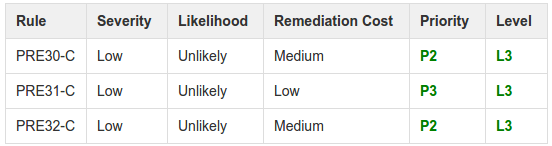
\includegraphics[width=.6\linewidth]{Figures/pre}
	\caption{Risk Assessment Summary of PRE }
	\label{fig:2}\cite{cert-c}
	
\end{figure}
\subsubsection{Declarations and initialization (02-DCL)}
 The rules and recommendations in this category mostly cover tricky semantics of the type system and variable declarations, such as implicit types, scopes, and conflicting linkage classifications. There are eight rules under this category. The risk analysis is shown in Figure \ref{fig:3}\cite{cert-c}
 \begin{itemize}
 	\item DCL30-C. Declare objects with appropriate storage durations

\item DCL31-C. Declare identifiers before using them

\item DCL36-C. Do not declare an identifier with conflicting linkage classifications

\item DCL37-C. Do not declare or define a reserved identifier

\item DCL38-C. Use the correct syntax when declaring a flexible array member

\item DCL39-C. Avoid information leakage in structure padding

\item DCL40-C. Do not create incompatible declarations of the same function or object

\item DCL41-C. Do not declare variables inside a switch statement before the first case label
\end{itemize}
\begin{figure}[H]
	
	
	\centering
	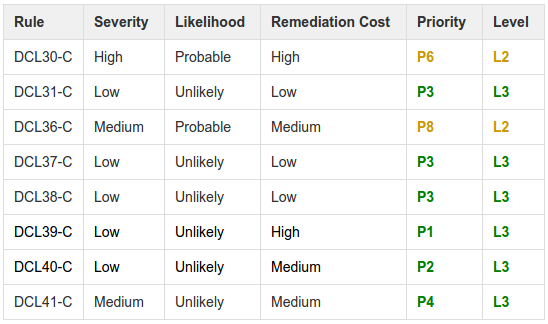
\includegraphics[width=.6\linewidth]{Figures/dcl}
	\caption{Risk Assessment Summary of DCL}
	\label{fig:3}
	
\end{figure}
\subsubsection{Expressions (03-EXP)} The rules and recommendations in this category are concerned with issues related to expressions, including (unspecified) evaluation order, type conversions, sizes of data types, general use of pointers, and so forth.There are fourteen  rules under this category. The risk analysis is shown in Figure \ref{fig:4}\cite{cert-c}
\begin{itemize}
	\item EXP30-C. Do not depend on the order of evaluation for side effects

\item EXP32-C. Do not access a volatile object through a non volatile reference

\item EXP33-C. Do not read uninitialized memory

\item EXP34-C. Do not dereference null pointers

\item EXP35-C. Do not modify objects with temporary lifetime

\item EXP36-C. Do not cast pointers into more strictly aligned pointer types

\item EXP37-C. Call functions with the correct number and type of arguments

\item EXP39-C. Do not access a variable through a pointer of an incompatible type

\item EXP40-C. Do not modify constant objects

\item EXP42-C. Do not compare padding data

\item EXP43-C. Avoid undefined behavior when using restrict-qualified pointers

\item EXP44-C. Do not rely on side effects in operands to size of, Align of, or Generic

\item EXP45-C. Do not perform assignments in selection statements

\item EXP46-C. Do not use a bitwise operator with a Boolean-like operand
\end{itemize}
\begin{figure}[H]
	
	
	\centering
	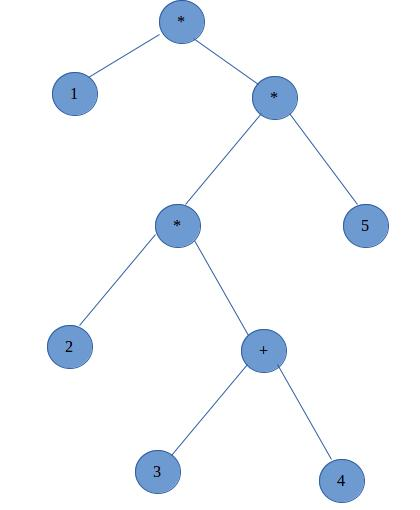
\includegraphics[width=.6\linewidth]{Figures/exp}
	\caption{Risk Assessment Summary of EXP}
	\label{fig:4}
	
\end{figure}
\subsubsection{Integers (04-INT)} The rules and recommendations in this category are concerned with issues related to proper handling of integers. The main emphasis for the rules is on avoiding overflows and wrap-around for very large or very small integer values. There are  seven  rules under this category. The risk analysis is shown in Figure \ref{fig:5}\cite{cert-c}
\begin{itemize}
	\item INT30-C. Ensure that unsigned integer operations do not wrap.
	\item INT31-C. Ensure that integer conversions do not result in lost or misinterpreted data.
	\item INT32-C. Ensure that operations on signed integers do not result in overflow.
	\item INT33-C. Ensure that division and remainder operations do not result in divide-by-zero errors.
	\item INT34-C. Do not shift an expression by a negative number of bits or by greater than or equal to the number of bits that exist in the operand.
	\item INT35-C. Use correct integer precisions.
	\item INT36-C. Converting a pointer to integer or integer to pointer
\end{itemize}
\begin{figure}[H]
	
	
	\centering
	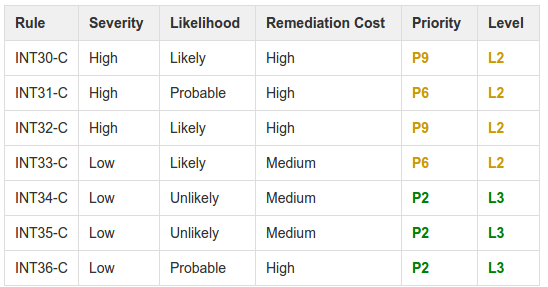
\includegraphics[width=.6\linewidth]{Figures/int}
	\caption{Risk Assessment Summary of INT}
	\label{fig:5}
	
\end{figure}
\subsubsection{Floating point (05-FLP)} The rules and recommendations in this category are concerned with issues relating to proper handling of floating point types: loss of precision, proper use of mathematical functions, and type conversion. There are five  rules under this category. The risk analysis is shown in Figure \ref{fig:6}\cite{cert-c}
\begin{itemize}
	\item FLP30-C. Do not use floating-point variables as loop counters
	
	\item FLP32-C. Prevent or detect domain and range errors in math functions
	
	\item FLP34-C. Ensure that floating-point conversions are within range of the new type
	
	\item FLP36-C. Preserve precision when converting integral values to floating-point type
	
	\item FLP37-C. Do not use object representations to compare floating-point values
\end{itemize}
\begin{figure}[H]
	
	
	\centering
	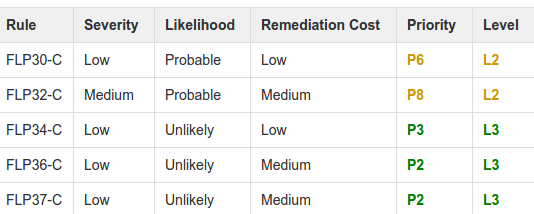
\includegraphics[width=.6\linewidth]{Figures/flp}
	\caption{Risk Assessment Summary of FLP}
	\label{fig:6}
	
\end{figure}
\subsubsection{Arrays (06-ARR)} The rules and recommendations in this category focus on avoiding out of bounds array indexing and pointer access to arrays. There are six rules under this category. The risk analysis is shown in Figure \ref{fig:7}\cite{cert-c}
\begin{itemize}
	\item ARR30-C. Do not form or use out-of-bounds pointers or array subscripts
	
	\item ARR32-C. Ensure size arguments for variable length arrays are in a valid range
	
	\item ARR36-C. Do not subtract or compare two pointers that do not refer to the same array
	
	\item ARR37-C. Do not add or subtract an integer to a pointer to a non-array object
	
	\item ARR38-C. Guarantee that library functions do not form invalid pointers
	
	\item ARR39-C. Do not add or subtract a scaled integer to a pointer
\end{itemize}
\begin{figure}[H]
	
	
	\centering
	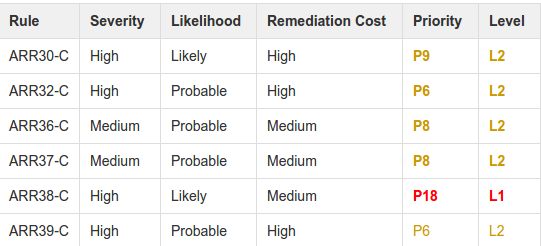
\includegraphics[width=.6\linewidth]{Figures/arr}
	\caption{Risk Assessment Summary of ARR}
	\label{fig:7}
	
\end{figure}
\subsubsection{Characters and strings (07-STR)} The rules and recommendations in this category are concerned with ensuring null termination of strings, proper size calculation of strings, and bounds checking for strings. There are six rules under this category. The risk analysis is shown in Figure \ref{fig:8}\cite{cert-c}
\begin{itemize}
	\item STR30-C. Do not attempt to modify string literals
	
	\item STR31-C. Guarantee that storage for strings has sufficient space for character data and the null terminator
	
	\item STR32-C. Do not pass a non-null-terminated character sequence to a library function that expects a string
	
	\item STR34-C. Cast characters to unsigned char before converting to larger integer sizes
	
	\item STR37-C. Arguments to character-handling functions must be representable as an unsigned char
	
	\item STR38-C. Do not confuse narrow and wide character strings and functions
\end{itemize}
\begin{figure}[H]
	
	
	\centering
	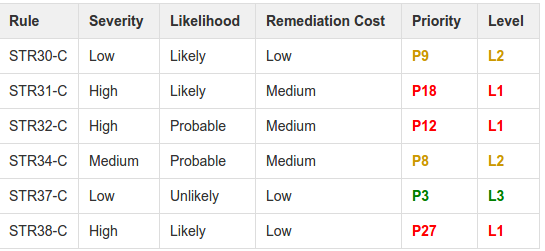
\includegraphics[width=.6\linewidth]{Figures/str}
	\caption{Risk Assessment Summary of STR}
	\label{fig:8}
	
\end{figure}
\subsubsection{Memory management (08-MEM)}  Implementing memory management correctly is notoriously difficult and even small bugs in this category are likely to result in a security vulnerability, e.g., a buffer overflow or a null pointer dereference. There are six rules under this category. The risk analysis is shown in Figure \ref{fig:9}\cite{cert-c}
\begin{itemize}
	\item MEM30-C. Do not access freed memory
	
	\item MEM31-C. Free dynamically allocated memory when no longer needed
	
	\item MEM33-C. Allocate and copy structures containing a flexible array member dynamically
	
	\item MEM34-C. Only free memory allocated dynamically
	
	\item MEM35-C. Allocate sufficient memory for an object
	
	\item MEM36-C. Do not modify the alignment of objects by calling realloc()
	
\end{itemize}
\begin{figure}[H]
	
	
	\centering
	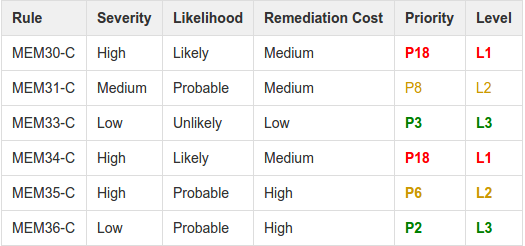
\includegraphics[width=.6\linewidth]{Figures/mem}
	\caption{Risk Assessment Summary of MEM}
	\label{fig:9}
	
\end{figure}
\subsubsection{Input-output (09-FIO)} The rules and recommendations in this category are mainly concerned with the proper use of library functions for (file) input and output, including proper opening and closing of files, creation of temporary files, as well as the secure creation of format strings. There are five rules under this category. The risk analysis is shown in Figure \ref{fig:10}\cite{cert-c}
\begin{itemize}
\item FIO30-C. Exclude user input from format strings

\item FIO32-C. Do not perform operations on devices that are only appropriate for files

\item FIO34-C. Distinguish between characters read from a file and EOF or WEOF

\item FIO37-C. Do not assume that fgets() or fgetws() returns a nonempty string when successful

\item FIO38-C. Do not copy a FILE object

\item FIO39-C. Do not alternately input and output from a stream without an intervening flush or positioning call

\item FIO40-C. Reset strings on fgets() or fgetws() failure

\item FIO41-C. Do not call getc(), putc(), getwc(), or putwc() with a stream argument that has side effects

\item FIO42-C. Close files when they are no longer needed

\item FIO44-C. Only use values for fsetpos() that are returned from fgetpos()

\item FIO45-C. Avoid TOCTOU race conditions while accessing files

\item FIO46-C. Do not access a closed file

\item FIO47-C. Use valid format strings	
\end{itemize}
\begin{figure}[H]
	
	
	\centering
	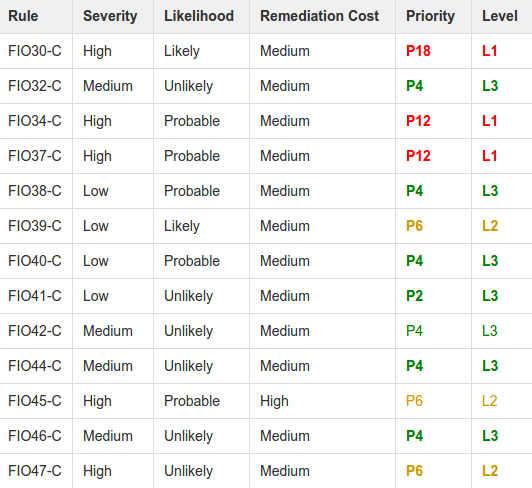
\includegraphics[width=.6\linewidth]{Figures/fio}
	\caption{Risk Assessment Summary of FIO}
	\label{fig:10}
	
\end{figure}
 
\subsubsection{Environment (10-ENV)} The rules and recommendations in this category are concerned with the proper handling of the execution environment, e.g., environment variables, and calls to external command processors. There are five rules under this category. The risk analysis is shown in Figure \ref{fig:11}\cite{cert-c}
\begin{itemize}
\item ENV30-C. Do not modify the object referenced by the return value of certain functions

\item ENV31-C. Do not rely on an environment pointer following an operation that may invalidate it

\item ENV32-C. All exit handlers must return normally

\item ENV33-C. Do not call system()

\item ENV34-C. Do not store pointers returned by certain functions
\end{itemize}
\begin{figure}[H]
	
	
	\centering
	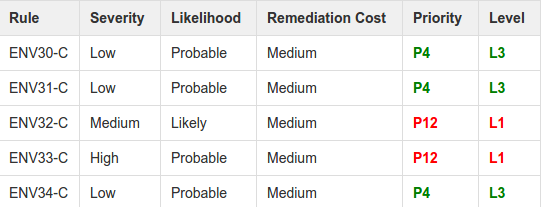
\includegraphics[width=.6\linewidth]{Figures/env}
	\caption{Risk Assessment Summary of ENV}
	\label{fig:11}
	
\end{figure}
\subsubsection{Signals (11-SIG)} The rules and recommendations in this category are concerned with raising and handling signals in a secure manner. There are four rules under this category. The risk analysis is shown in Figure \ref{fig:12}\cite{cert-c}
	\begin{itemize}
		\item SIG30-C. Call only asynchronous-safe functions within signal handlers
		
		\item SIG31-C. Do not access shared objects in signal handlers
		
		\item SIG34-C. Do not call signal() from within interruptible signal handlers
		
		\item SIG35-C. Do not return from a computational exception signal handler
	\end{itemize}
	\begin{figure}[H]
		
		
		\centering
		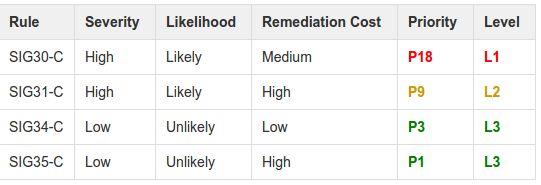
\includegraphics[width=.6\linewidth]{Figures/sig}
		\caption{Risk Assessment Summary of SIG}
		\label{fig:12}
		
	\end{figure}
	\subsubsection{Error handling (12-ERR)} The rules and recommendations in this category are concerned with detecting and handling errors and proper handling of the errno variable.  There are four rules under this category. The risk analysis is shown in Figure \ref{fig:13}\cite{cert-c}
	\begin{itemize}
		\item ERR30-C. Set errno to zero before calling a library function known to set errno, and check errno only after the function returns a value indicating failure
		
		\item ERR32-C. Do not rely on indeterminate values of errno
		
		\item ERR33-C. Detect and handle standard library errors
			\end{itemize}
			\begin{figure}[H]
				
				
				\centering
				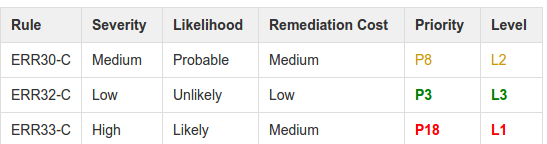
\includegraphics[width=.6\linewidth]{Figures/err}
				\caption{Risk Assessment Summary of ERR}
				\label{fig:13}
				
			\end{figure}
			\subsubsection{Concurrency (14-CON)} The rules and recommendations in this category are general observations concerning concurrent programming such as avoiding race conditions and deadlocks by locking in a predefined order.There are twelve rules under this category. The risk analysis is shown in Figure \ref{fig:14}
			\begin{itemize}
				\item CON30-C. Clean up thread-specific storage
				
				\item CON31-C. Do not destroy a mutex while it is locked
				
				\item CON32-C. Prevent data races when accessing bit-fields from multiple threads
				
				\item CON33-C. Avoid race conditions when using library functions
				
				\item CON34-C. Declare objects shared between threads with appropriate storage durations
				
				\item CON35-C. Avoid deadlock by locking in a predefined order
				
				\item CON36-C. Wrap functions that can spuriously wake up in a loop
				
				\item CON37-C. Do not call signal() in a multithreaded program
				
				\item CON38-C. Preserve thread safety and liveness when using condition variables
				
				\item CON39-C. Do not join or detach a thread that was previously joined or detached
				
				\item CON40-C. Do not refer to an atomic variable twice in an expression
				
				\item CON41-C. Wrap functions that can fail spuriously in a looph
			\end{itemize}
			\begin{figure}[H]
				
				
				\centering
				\includegraphics[width=.6\linewidth]{Figures/con}
				\caption{Risk Assessment Summary of CON}
				\label{fig:14}
				
			\end{figure}
			\subsubsection{Miscellaneous (49-MSC)} The rules and recommendations in this category are those that do not fit into any other category.There are seven rules under this category. The risk analysis is shown in Figure \ref{fig:15}\cite{cert-c}
				\begin{itemize}
					\item MSC30-C. Do not use the rand() function for generating pseudorandom numbers
					
					\item MSC32-C. Properly seed pseudorandom number generators
					
					\item MSC33-C. Do not pass invalid data to the asctime() function
					
					\item MSC37-C. Ensure that control never reaches the end of a non-void function
					
					\item MSC38-C. Do not treat a predefined identifier as an object if it might only be implemented as a macro
					
					\item MSC39-C. Do not call va\_arg() on a va\_list that has an indeterminate value
					
					\item MSC40-C. Do not violate constraints
				\end{itemize}
				\begin{figure}[H]
					
					
					\centering
					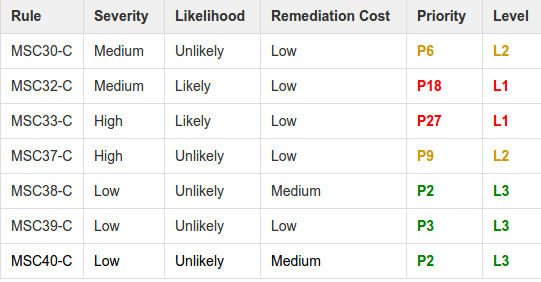
\includegraphics[width=.6\linewidth]{Figures/msc}
					\caption{Risk Assessment Summary of MSC}
					\label{fig:15}
					
				\end{figure}
\subsubsection{POSIX (50-POS)} The rules and recommendations in this category cover compliance with and proper use of POSIX. There are four rules under this category. The risk analysis is shown in Figure \ref{fig:16}\cite{cert-c}
	\begin{itemize}
		\item POS30-C. Use the readlink() function properly
		
		\item POS33-C. Do not use vfork()
		
		\item POS34-C. Do not call putenv() with a pointer to an automatic variable as the argument
		
		\item POS35-C. Avoid race conditions while checking for the existence of a symbolic link
		
		\item POS36-C. Observe correct revocation order while relinquishing privileges
		
		\item POS37-C. Ensure that privilege relinquishment is successful
		
		\item POS38-C. Beware of race conditions when using fork and file descriptors
		
		\item POS39-C. Use the correct byte ordering when transferring data between systems
		
		\item POS44-C. Do not use signals to terminate threads
		
		\item POS47-C. Do not use threads that can be canceled asynchronously
		
		\item POS48-C. Do not unlock or destroy another POSIX thread's mutex
		
		\item POS49-C. When data must be accessed by multiple threads, provide a mutex and guarantee no adjacent data is also accessed
		
		\item POS50-C. Declare objects shared between POSIX threads with appropriate storage durations
		
		\item POS51-C. Avoid deadlock with POSIX threads by locking in predefined order
		
		\item POS52-C. Do not perform operations that can block while holding a POSIX lock
		
		\item POS53-C. Do not use more than one mutex for concurrent waiting operations on a condition variable
		
		\item POS54-C. Detect and handle POSIX library errors
	\end{itemize}
	\begin{figure}[H]
		
		
		\centering
		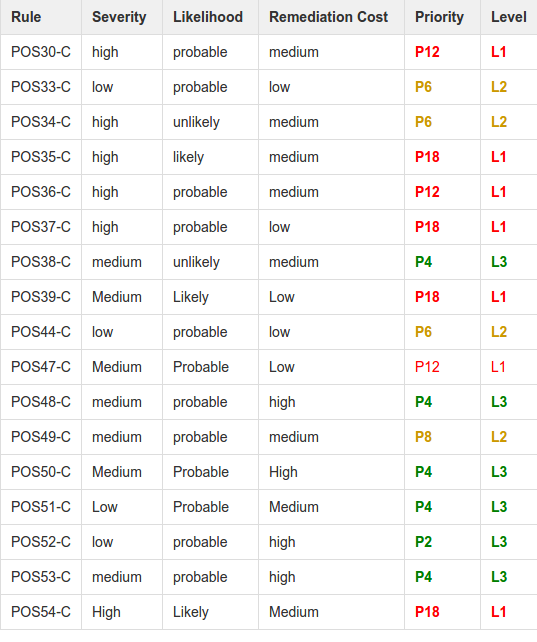
\includegraphics[width=.6\linewidth]{Figures/pos}
		\caption{Risk Assessment Summary of POS}
		\label{16}
		
	\end{figure}
 


% -eof-


% -eof-
